\chapter{Conclusions et perspectives}
\renewcommand\chapterillustration{CON/CON}
\ThisULCornerWallPaper{1}{\chapterillustration}
%\minitoc
\vspace*{-0.5cm}
\lettrine[lines=4, slope=-0.5em,nindent=10pt]{A}{vec} la mise à niveau du LHC en HL-LHC prévu pour 2026, la luminosité instantanée et le pile-up des événements vont augmenter de façon significative. Afin de faire face à cette augmentation du taux de collisions, le détecteur CMS doit être lui aussi mis à niveau. De nombreux changement dans presque tous les ses sous-détecteurs sont prévus.

Dans le trajectographe à muons, et notamment dans les bouchons, le programme d'amélioration prévois, entre autres, d'instrumenter les zones RE3/1 et RE4/1 avec des RPC de nouvelle générations appellés iRPC. Ces zones initialement prévus pour être instrumenter par des RPC dès le début de la construction de CMS en sont toujours dépourvu en raison du flux importants de particules les traversant.

Fort des connaissances et de l'expertise acquises sur les GRPC, depuis plus de dix ans, lors de la construction du SDHCAL pour ILC, l'IPNL à décidé de s'investir dans la mise à niveau des bouchons de CMS. Une collaboration avec nos collègues chinois de Tsinghua a permis de proposer l'utilisation de verre de basse résistivité \SI{e10}{\ohm\per\centi\meter} comme électrodes pour les chambres RPC à instrumenter dans les zones RE3/1 ET RE4/1. 

Cette thèse a eu pour but de caractériser ces verres et de vérifier s'ils pouvait être utiliser pour la construction de chambre RPC en vu de l'instrumentation de ces zones. Pour cela, de nombreux tests en faisceaux au PS, SPS, et GIF++ ont été réalisés. Ces tests on montrés que ce type de verres pouvait résister de des flux de particules très importants pour des RPC \SI{3}{\kilo\hertz\per\square\centi\meter}. Nous avons également démontré qu'il était possible de construire des chambres de grande taille (RE1/1) avec ces verres, limité par leur procédé de fabrication à une surface de \SI{32}{\centi\meter}$\times$\SI{30}{\centi\meter}. Cependant, ces verres semblent inadapté au mélange de gaz utilisé dans CMS. Des test effectués à Lyon et au CERN tendent à démontrer que ce type de verre nécessiteraient un mélange gazeux comportant une proportion plus importante de \chemform{SF_6} que celui utilisé dans CMS afin de réduire significativement le bruit. De plus, étant donné les problèmes rencontrés sur notre installation au GIF++, nous n'avons pas était en mesure de démontrer que ces verres résiste à \num{10} ans d'opération de CMS.

Parallèlement, nous avons proposé un nouveau type de PCB basé des ASIC PETIROC2 et permettant de lire les strips des chambres des deux côtés. Ce type de lecture permet de supprimer le partitionnement et permet également d'obtenir la position du hits le long des strips. Des tests effectué en Mai 2017 sur la ligne H4 ont ainsi montrés que cette position pouvait être connue avec une résolution de l'autre de \SI{1.8}{\centi\meter} contre une résolution correspondante à la longueur des strips actuellement. Ces résultats, très satisfaisant, malgré certains problème sur le PCB et l'absence de calibration des strips ont amené la communauté muons de CMS à choisir cette méthode de lecture comme solution privilégié pour le TDR actuellement en cours de rédaction.

De nombreuses améliorations et adaptations de cette électronique sont dés à présent prévu. La valeur minimale de la gamme dynamique du seuil va être baissé afin de déclencher sur des signaux de \SI{10}{\femto\coulomb}, la technologie \chemform{SiGe} à \SI{350}{\nano\meter} va être remplacer par une technologie CMOS à \SI{130}{\nano\meter} par l'entreprise \textit{Taiwan Semiconductor Manufacturing Company} (TSMC) afin de rendre cette ASIC plus tolérant au radiation. Son nombres de voies d'entrées va également être augmenté et passer de \num{32} à \num{64}.

Les mezzanines s'occupant des TDC vont être remplacé par des FPGA. Une alternative permettant d'intégrer les TDC directement dans les ASIC est également à l'étude. Cette solution, présente l'avantage de diminuer la consommation électrique et évite les problèmes de routage des données; elle reposera sur des TDC utilisant le principe de Vernier (cf.fig~\ref{vernier}). Ce type de TDC utilise deux oscillateur de fréquence très proche l'une de l'autre afin de mesurer le temps.

\begin{figure}[ht!]
	\centering
	\subfloat[Schèma de principe du TDC de type Vernier.]{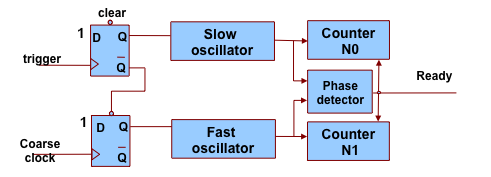
\includegraphics[width=0.49\textwidth]{CON/Vernier1.png}}
	\hfill
	\subfloat[Diagramme temporelle du principe de Vernier.]{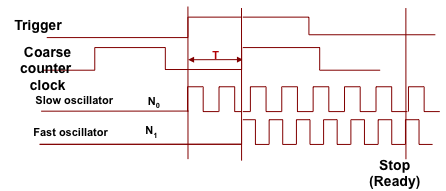
\includegraphics[width=0.49\textwidth]{CON/Vernier2.png}}
	\label{vernier}
	\caption{Schéma de principe et diagramme temporel du principe des TDC utilisant le principe de Vernier. Le temps calculée par le TDC est donnée par $T=N_0T_{slow}-N_1T_{fast}$.}
\end{figure}

Toute cette électronique est placé sur une mezzanine fixée directement sur les chambres (cf.fig~\ref{chamber}). Des câbles coaxiaux sont soudés à l'extremité des strips d'un côté et sont relié de l'autre à une carte, raccordée à la mezzanine qui permet, pour chaque câble d'adapter l'impédance à celle des voies d'entrée des ASIC ($\sim$\SI{200}{\ohm}).  

\begin{figure}[ht!]
	\centering
	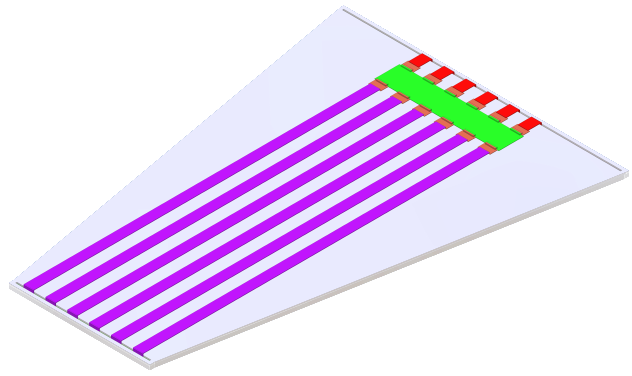
\includegraphics[width=0.50\textwidth]{CON/chambre.png}
	\captionof{figure}{Schéma d'une chambre iRPC avec l'électronique PETIROC2. La mezzanine est en vert. Les câbles coaxiaux venant des deux côtés des strips ( en violet et en rouge) sont connectés à la mezzanine par des cartes adaptatrices d'impédance (en orange). Le détecteur et le PCB avec les strips est à l'intérieur de la mécanique est ne sont pas visible.}
	\label{chamber}
\end{figure}

Les mezzanine seront relié à la DAQ par des \textit{Low power GigaBit Transceiver} (LpGBT) qui assureront également la connexion entre les ASIC et les TDC (cf.fig~\ref{chambres}). 

\begin{figure}[ht!]
	\centering
	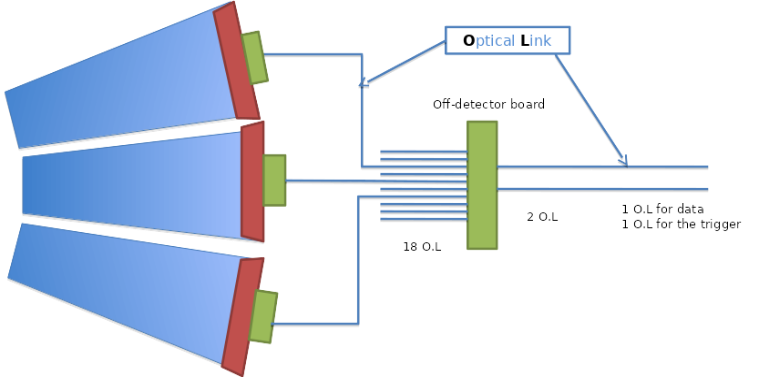
\includegraphics[width=0.70\textwidth]{CON/chambres.png}
	\captionof{figure}{Schéma du système DAQ des nouvelles chambres.}
	\label{chambres}
\end{figure}

Des prototypes de PCB comportant \num{96} strips et faisant la taille d'une demie chambre RE3/1 en $\phi$ \footnote{Ceci est nécessaire car la fabrication de PCB de grande taille est aujourd'hui très compliqué.} (cf.fig~\ref{proto}) ont été fabriqué et sont en phase de test à Lyon. Un autre type incorporants les retours des strips directement dans le PCB et ne nécessitant donc pas de souder des câbles coaxiaux aus strips est également à l'étude.

\begin{figure}[ht!]
	\centering
	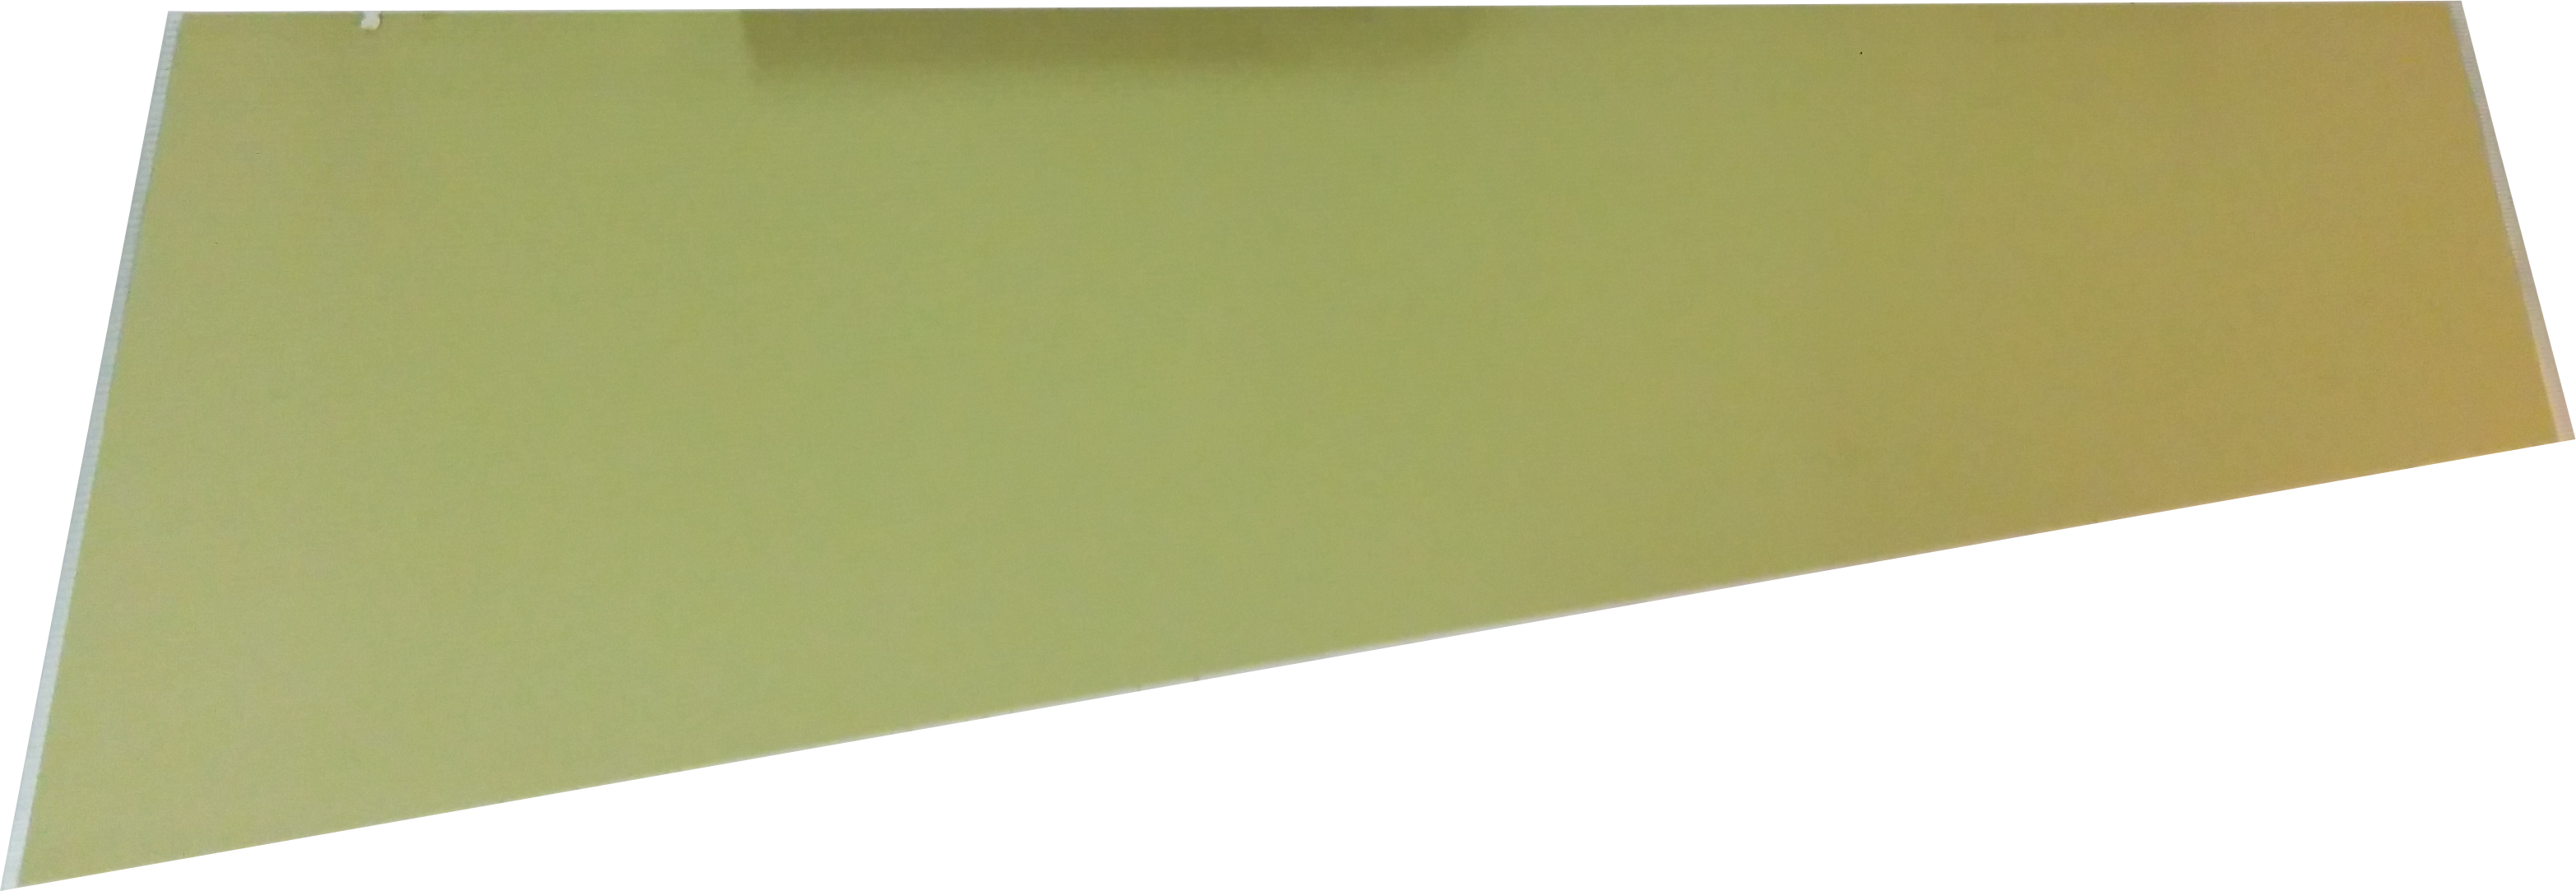
\includegraphics[width=0.75\textwidth]{CON/proto.png}
	\captionof{figure}{Le prototype de PCB avec lecture des strips des deux côtés.}
	\label{proto}
\end{figure}